\documentclass{article}
\usepackage{amsmath}
\usepackage{amsthm}
\usepackage{amsfonts}
\usepackage{amssymb}
\usepackage{bbold}
\usepackage{dsfont}
\usepackage{graphicx}
\usepackage{cleveref}
\usepackage{bm}
\usepackage{booktabs}
\usepackage{siunitx}
\usepackage{xcolor}
\usepackage[utf8]{inputenc}
\usepackage[english]{babel}
\newtheorem{definition}{Definition}
\newtheorem{example}{Example}
\newcommand{\exP}[1]{\mathrm{e}^{#1}}
\newcommand{\dif}{\mathrm{d}}
\renewcommand{\vec}[1]{\mathbf{#1}}
\newcommand{\pdagger}{{\phantom{\dagger}}}
\newcommand{\state}[1]{\vert #1\rangle}
\newcommand{\cstate}[1]{\langle #1\vert}
\newcommand{\tr}[1]{\mathrm{tr}\left\{#1\right\}}
\newcommand{\trs}[2]{\, \mathrm{tr}_{#1}\{#2\}}
\newcommand{\expc}[3]{\langle #1\vert #2 \vert #3\rangle}
\usepackage[doi=false,url=false,isbn=false,backend=bibtex,style=nature,natbib=true,sorting=none]{biblatex}
\bibliography{bib.bib}
\usepackage{geometry}
\geometry{
	a4paper,
	total={170mm,257mm},
	left=20mm,
	top=10mm,
	right=20mm,
	bottom=15mm
}
\begin{document}
\title{Report 8}
\author{Rudolf Smorka}
\maketitle
\section{Parameters}
We consider Fransson's model, which describes electrons or excitons on sites of a helical molecule. The Hamiltonian of this model consists of an electronic part, which incorporates electron hopping and static spin-orbit coupling 
\begin{equation}
	\begin{split}
		\hat{H}_\mathrm{el} &= \sum_{j,\sigma} \varepsilon_{j\sigma}^\pdagger \hat{d}_{j\sigma}^\dagger \hat{d}_{j\sigma}^\pdagger - t_0 \sum_{j\sigma} (\hat{d}_{j\sigma}^\dagger \hat{d}_{j+1,\sigma}^\pdagger + \mathrm{h.c.}) +\\& \lambda_0^\pdagger\sum_{j\sigma\sigma'} (i\hat{d}_{j\sigma}^\dagger (\vec{v}_j^{(+)}\cdot \bm{\sigma})_{\sigma\sigma'}^\pdagger \hat{d}_{j+2,\sigma'}^\pdagger + \mathrm{h.c.}),
	\end{split}
\end{equation}
the coupling between electrons and vibrations
\begin{align}
	\hat{H}_\mathrm{el-ph} &= - t_1^\pdagger \sum_{j,\sigma}  \hat{d}_{j\sigma}^\dagger \hat{d}_{j+1\sigma}^\pdagger (\hat{a}_{j}^\dagger + \hat{a}_{j}^\pdagger) \\ & + \lambda_1^\pdagger\sum_{j,\sigma,\sigma'} (i \hat{d}_{j\sigma}^\dagger (\vec{v}_j^{(+)} \cdot \bm{\sigma})_{\sigma\sigma'}^\pdagger \hat{d}_{j+2\sigma'}^\pdagger +\mathrm{h.c.})(\hat{a}_{j}^\dagger + \hat{a}_{j}^\pdagger),\label{eq:HelPh}
\end{align}
and the vibrational part
\begin{equation}
	\hat{H}_\mathrm{ph} = \sum_{j} \omega_{j}^\pdagger \hat{a}_{j}^\dagger \hat{a}_{j}^\pdagger.
	\label{eq:HPh} 
\end{equation}
The molecule is coupled to two leads of non-interacting electrons. The left lead is spin-polarized, characterized by $P$. The effect of this spin polarization is taken into account by making the leads spectral function (which we take to be constant) spin-dependent
\begin{equation}
	\Gamma_L= \Gamma_0 (1+P\sigma^z)
\end{equation}
In the following, we use the parameters:
\begin{align*}
	\varepsilon_0 &= -\SI{240}{\milli\electronvolt}\\
	\omega_0 &= \SI{50}{\milli\electronvolt}\\
	t_0 &= \SI{40}{\milli\electronvolt}\\
	t_1 &= 4,\SI{20}{\milli\electronvolt}\\
	\lambda_0 &= \SI{1}{\milli\electronvolt}\\
	\lambda_1 &= 0.1,\SI{1}{\milli\electronvolt}\\
	\Gamma &= \SI{10}{\milli\electronvolt}\\
	V 	&= \SI{480}{\milli\volt}\\
	T &= \SI{25}{\milli\electronvolt}.
\end{align*}
Within the TT-HEOM, the number of vibrational states is $n_\mathrm{vib}=30$. In both TT-HEOM and Ehrenfest-HEOM, the number of Pad\'{e} poles is $N_p = 10$. The Ehrenfest results are obtained by averaging over $12000$ trajectories with vibrational positions and momenta sampled from the thermal Wigner distribution at time $t=0$.
\clearpage
\section{Spinless Peierls model $L=2$}
\subsection{$\omega_0 = \SI{2}{\milli\electronvolt}, t_1=\SI{4}{\milli\electronvolt}$}
\begin{figure}[!h]
	\centering
	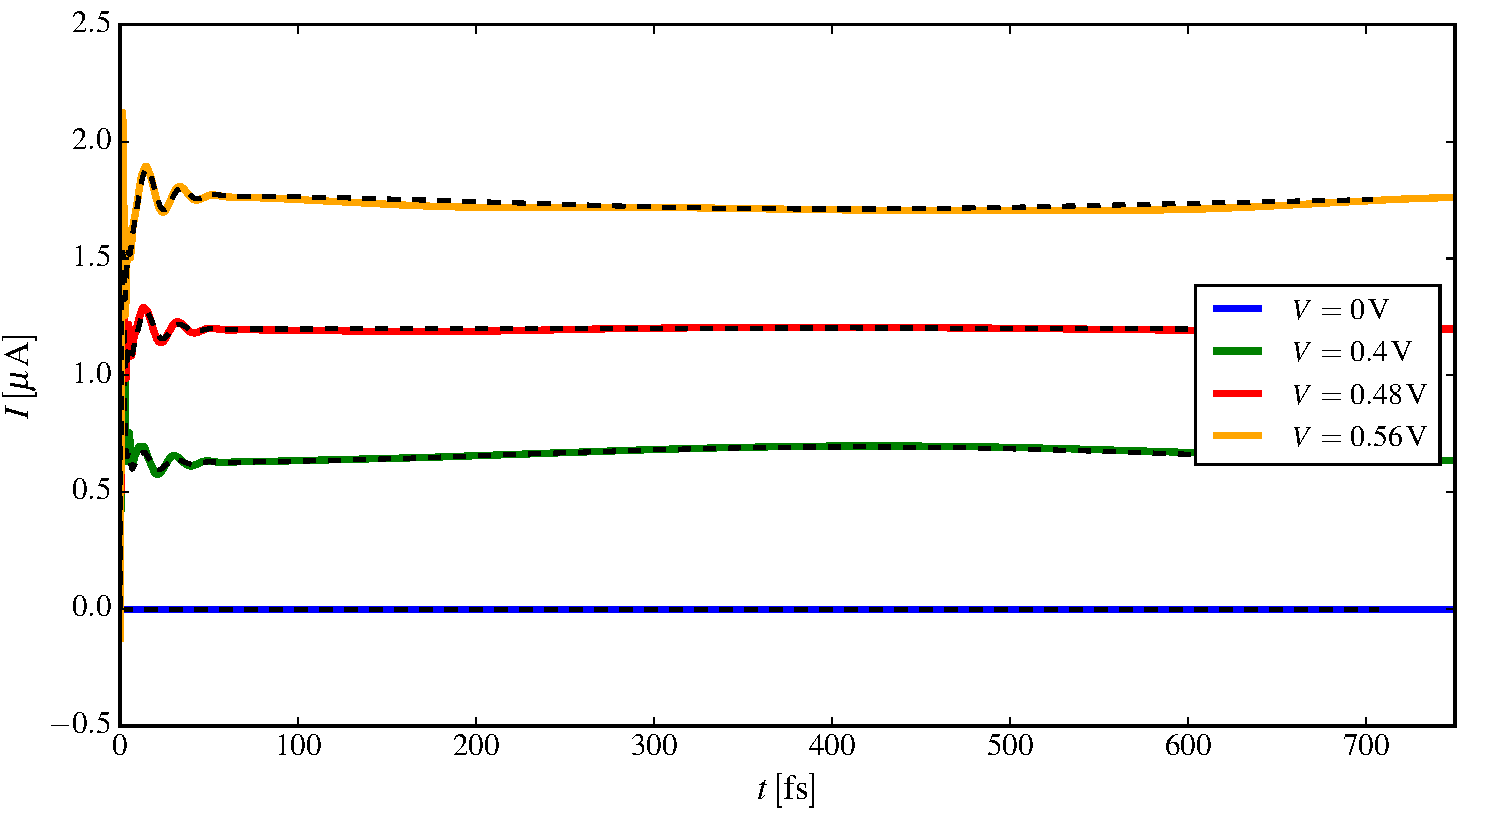
\includegraphics[width=0.8\textwidth]{figs/Peierls_L2_FranssonParams_Vvar_comparison_currents.pdf}
	\caption{Colored lines: MF-HEOM. Black dashed lines: TT-HEOM}
\end{figure}
\begin{figure}[!h]
	\centering
	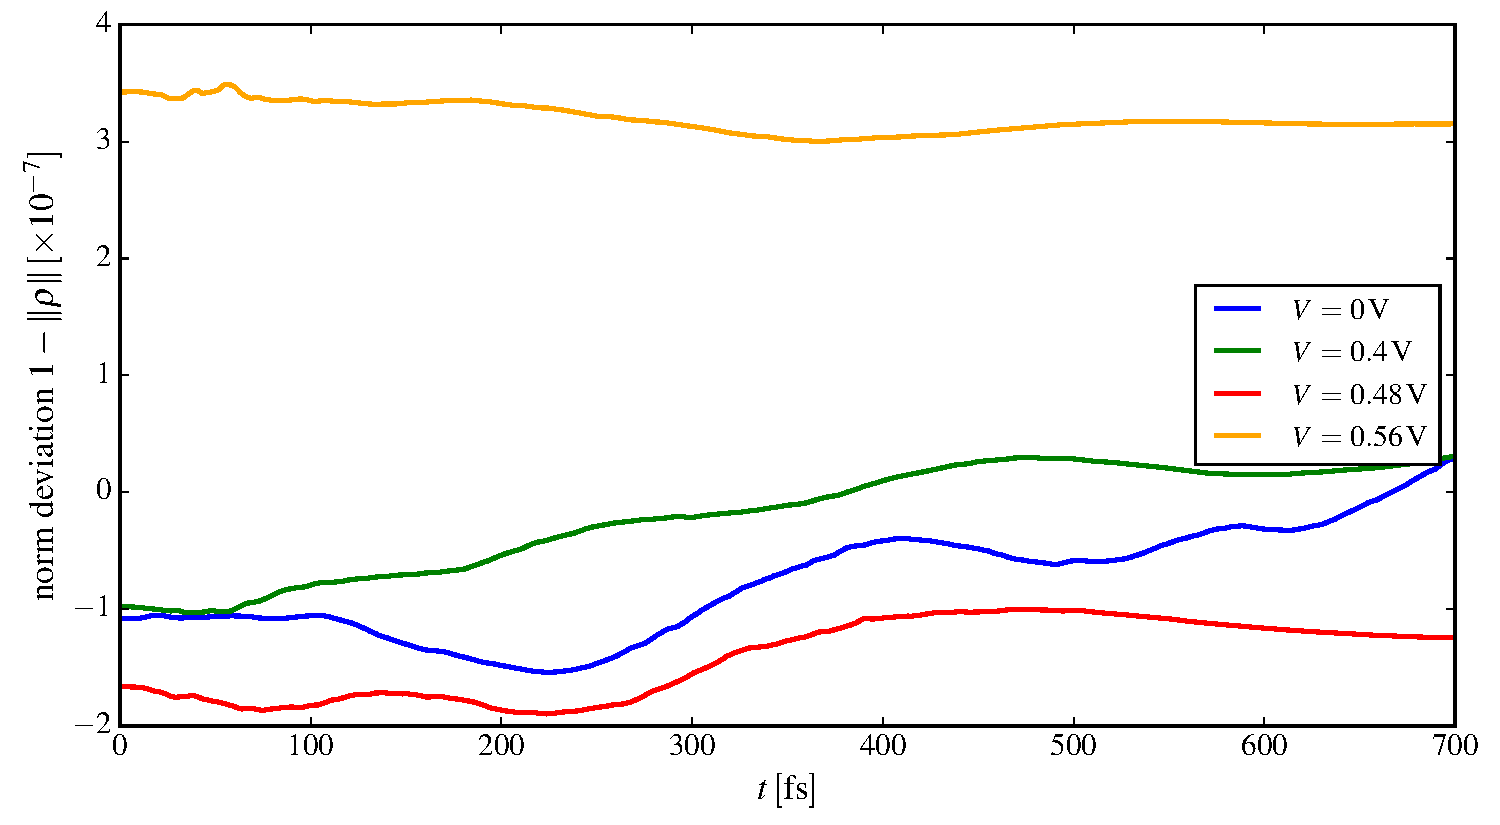
\includegraphics[width=0.8\textwidth]{figs/Peierls_L2_w0_0.002_t1_0.004_Vvar_norm.pdf}
\end{figure}
\begin{figure}[!h]
	\centering
	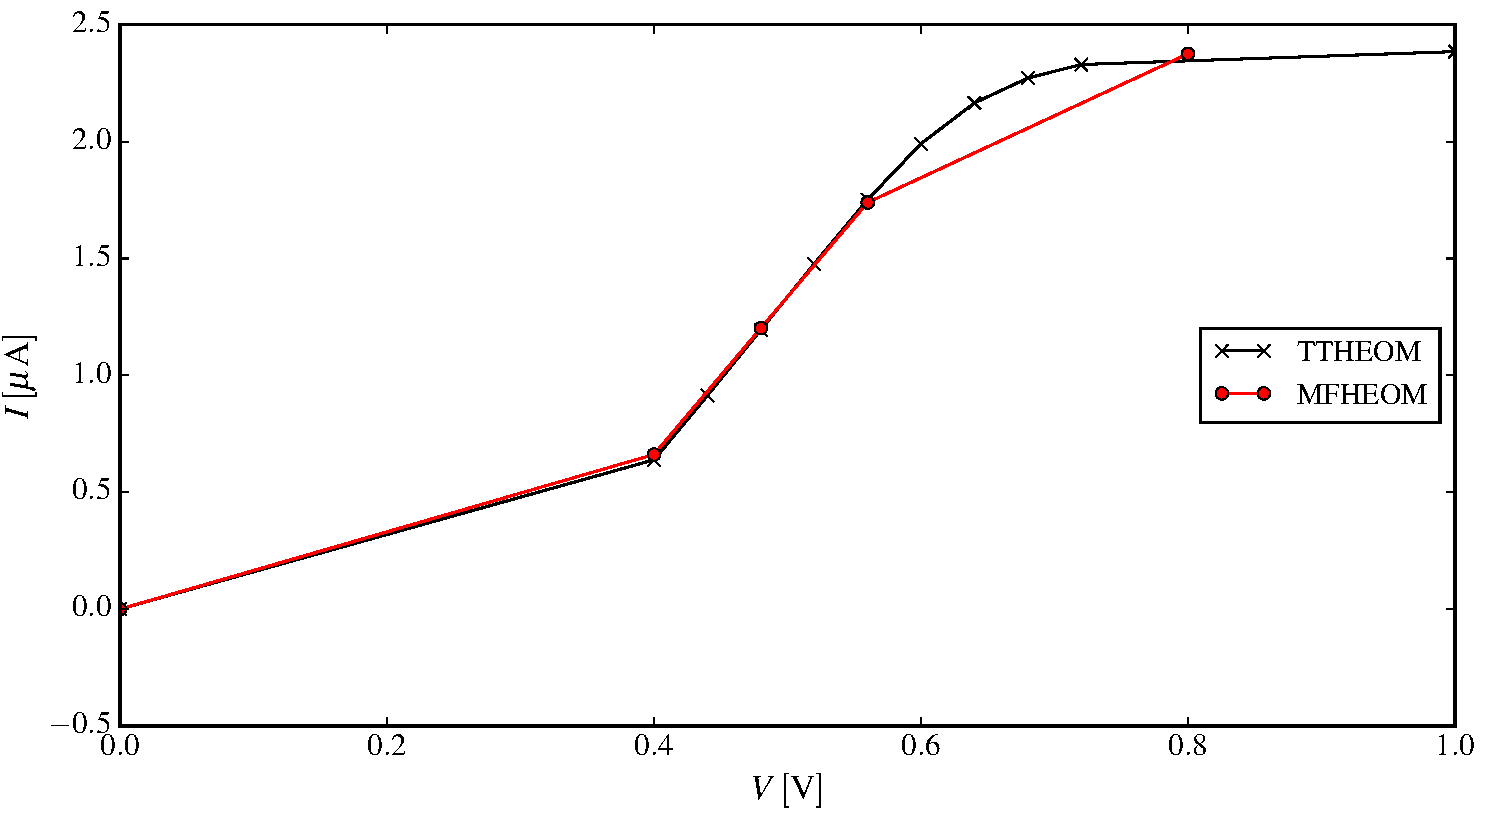
\includegraphics[width=0.8\textwidth]{figs/Peierls_L2_w0_0.002_t1_0.004_I_V_comparison.pdf}
\end{figure}
\clearpage
\subsection{$\omega_0 = \SI{50}{\milli\electronvolt}, t_1=\SI{4}{\milli\electronvolt}$}
\begin{figure}[!h]
	\centering
	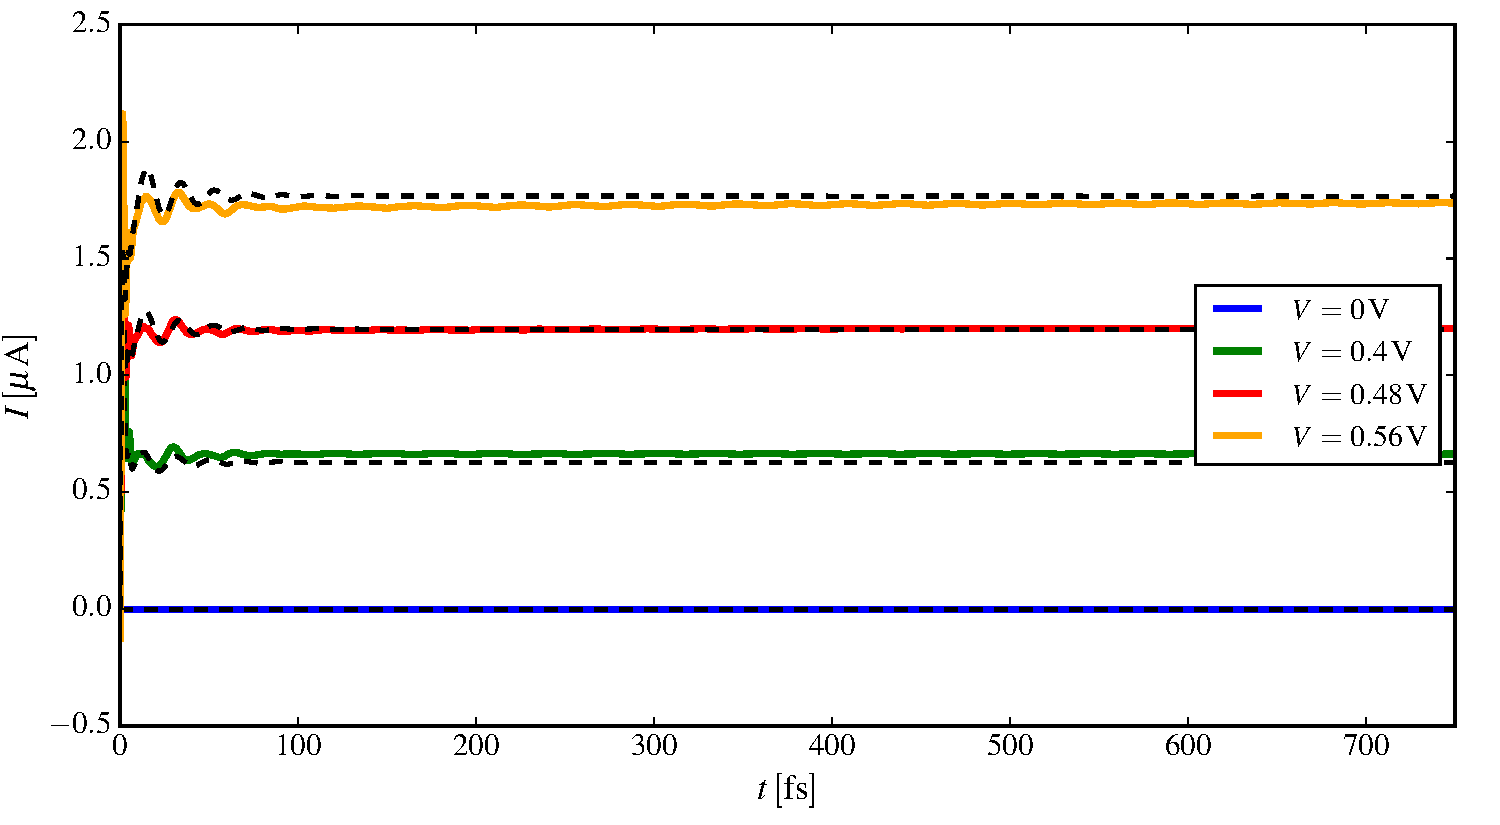
\includegraphics[width=0.8\textwidth]{figs/Peierls_L2_w0_0.05_t1_0.004_Vvar_comparison_currents.pdf}
	\caption{Colored lines: MF-HEOM. Black dashed lines: TT-HEOM}
\end{figure}
\begin{figure}[!h]
	\centering
	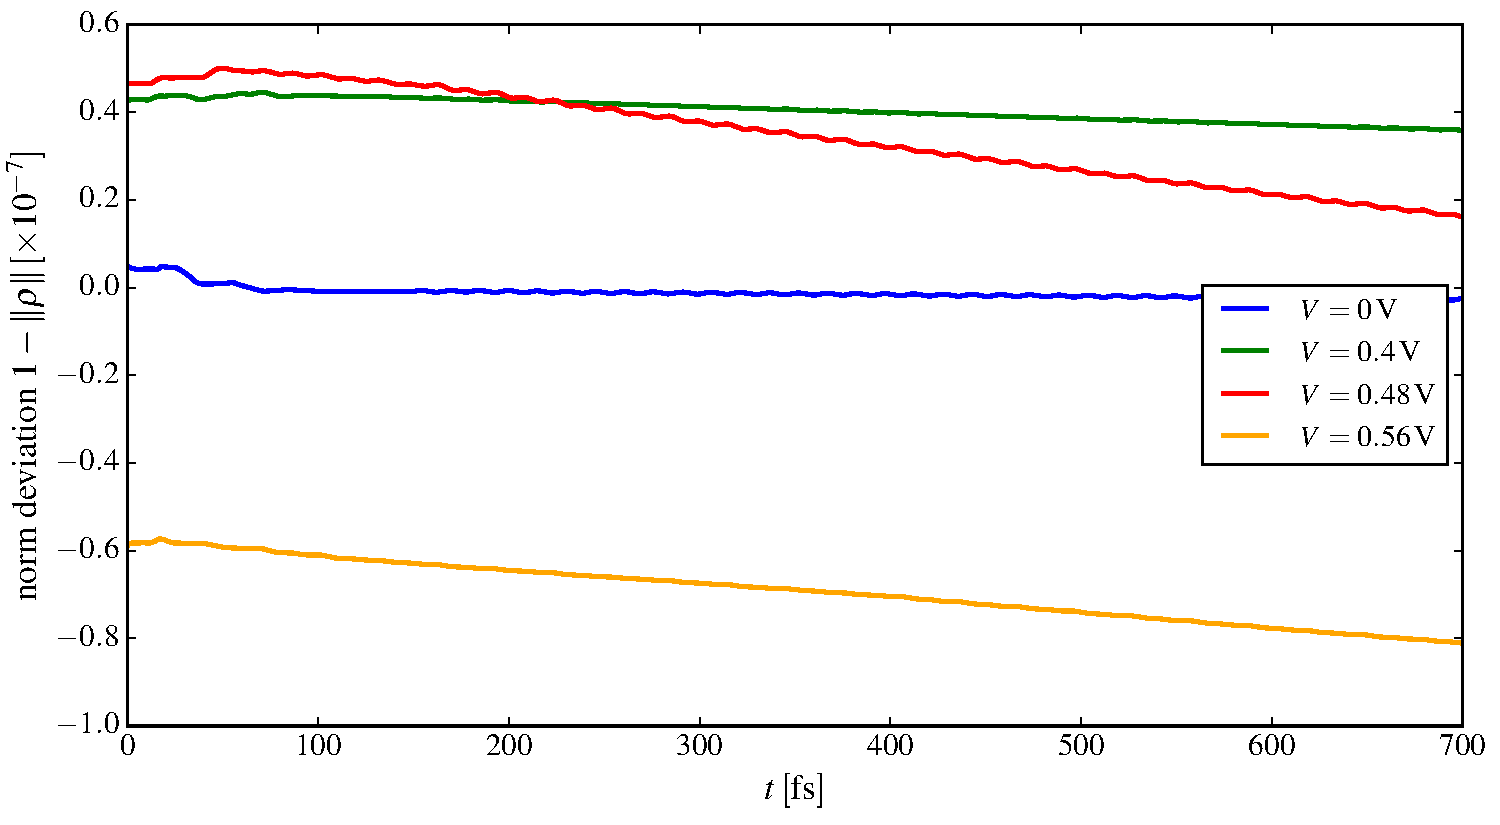
\includegraphics[width=0.8\textwidth]{figs/Peierls_L2_w0_0.05_t1_0.004_Vvar_norm.pdf}
\end{figure}
\begin{figure}[!h]
	\centering
	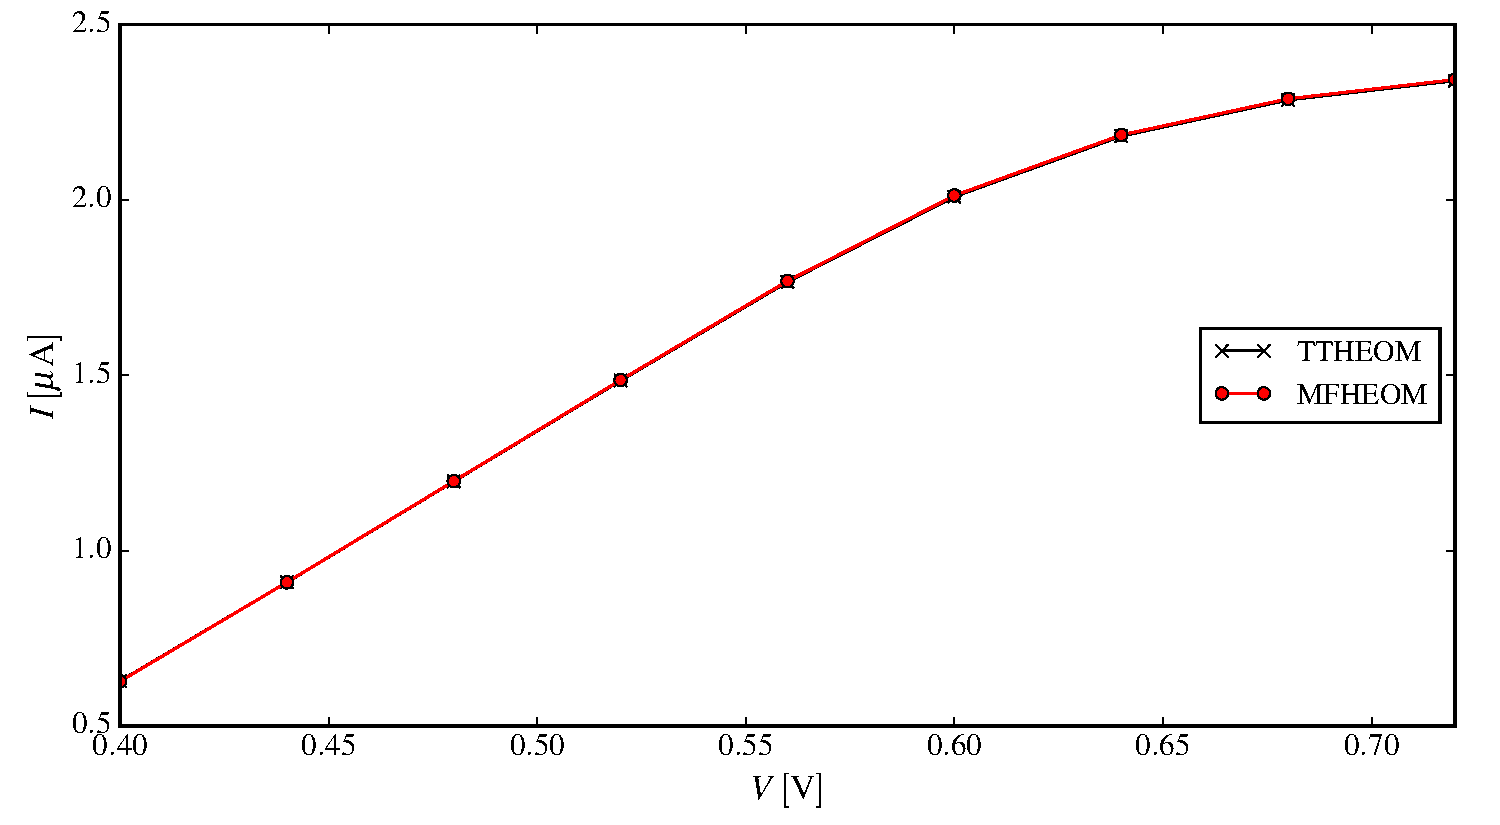
\includegraphics[width=0.8\textwidth]{figs/Peierls_L2_w0_0.05_t1_0.004_I_V_comparison.pdf}
\end{figure}
\clearpage
\subsection{$\omega_0 = \SI{100}{\milli\electronvolt}, t_1=\SI{4}{\milli\electronvolt}$}
\begin{figure}[!h]
	\centering
	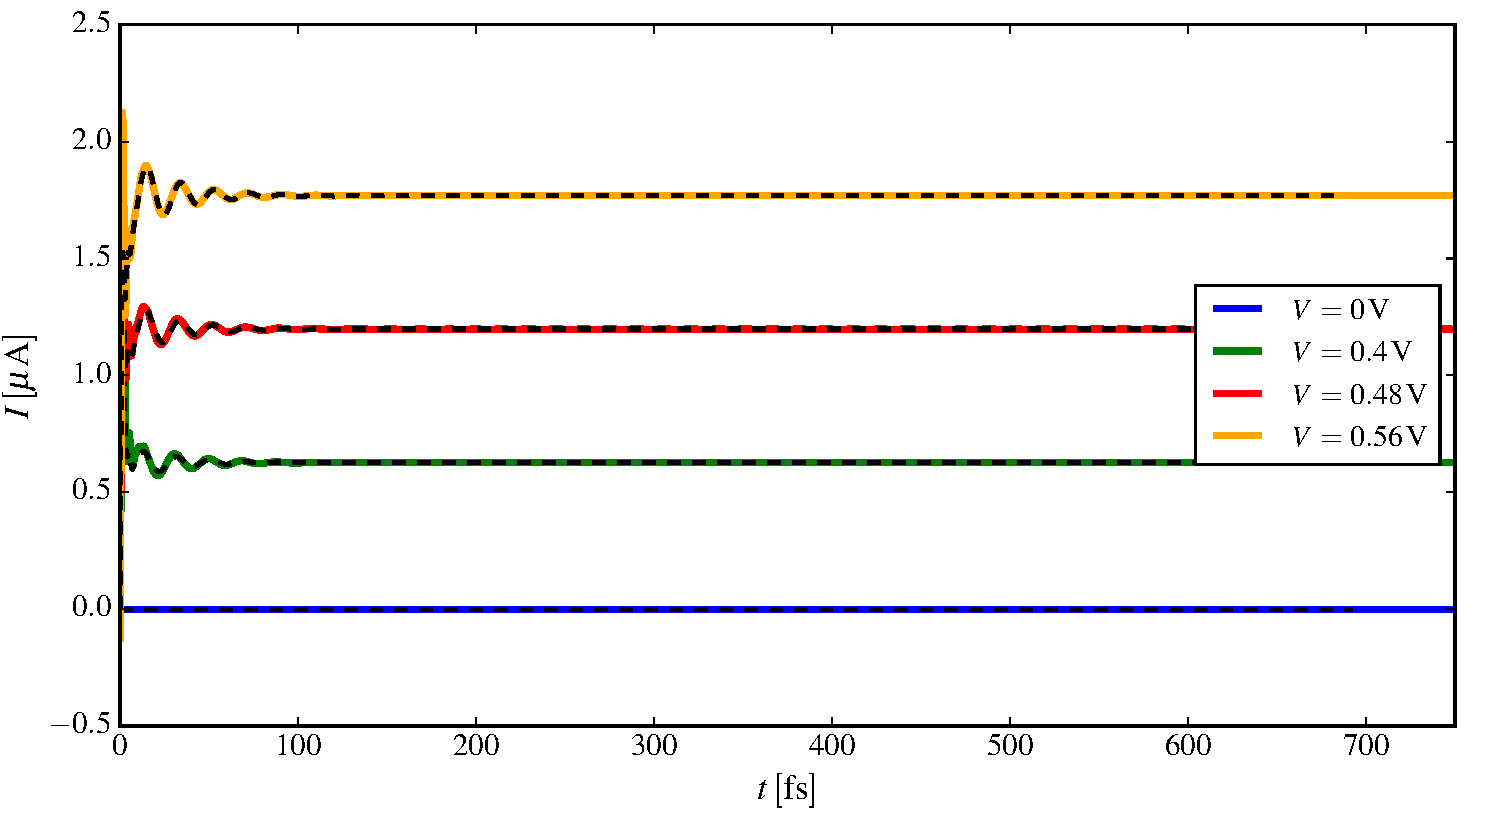
\includegraphics[width=0.8\textwidth]{figs/Peierls_L2_w0_0.1_t1_0.004_Vvar_comparison_currents.pdf}
	\caption{Colored lines: MF-HEOM. Black dashed lines: TT-HEOM}
\end{figure}
\begin{figure}[!h]
	\centering
	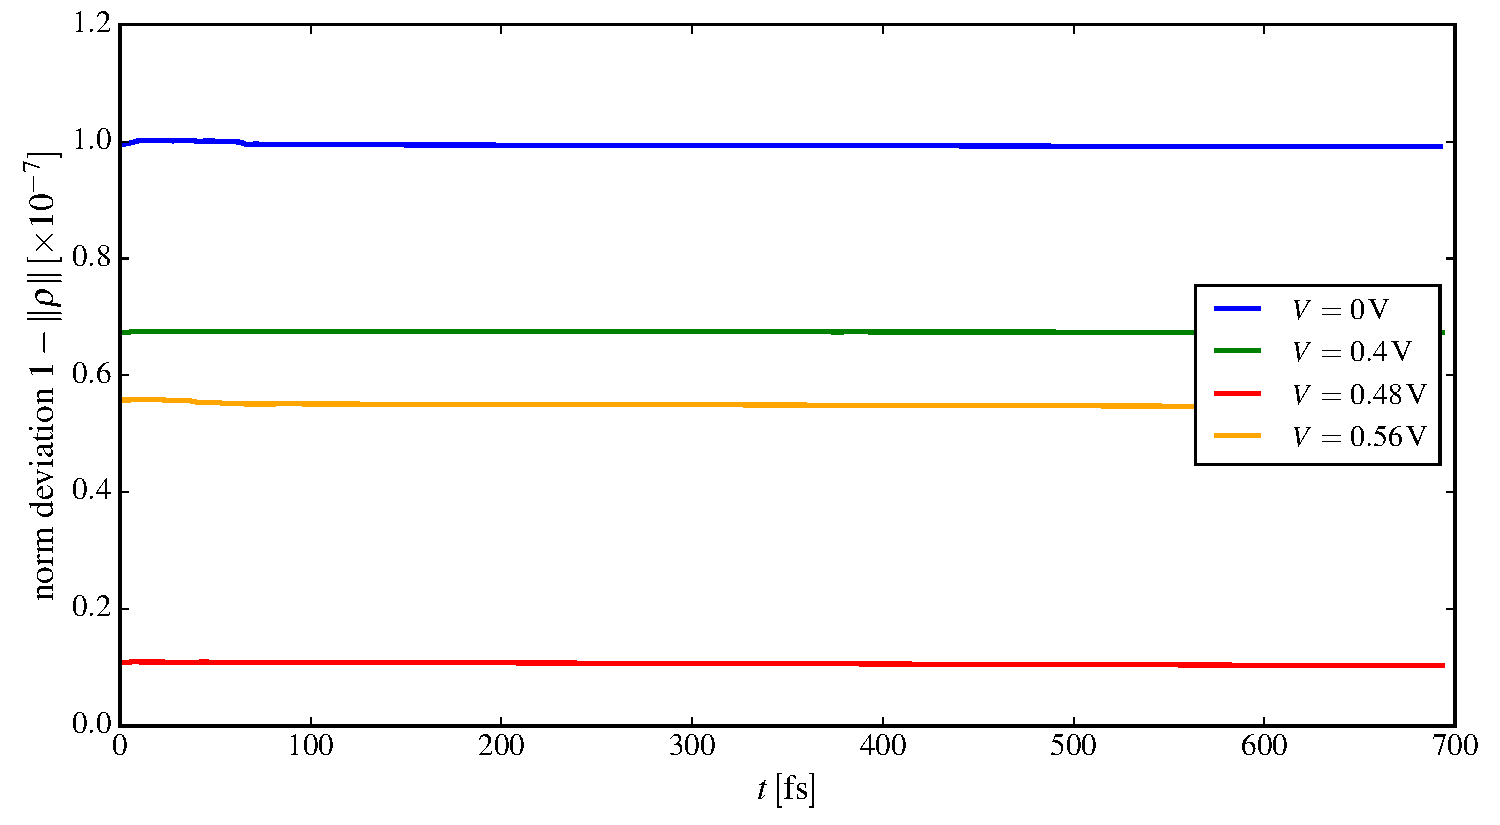
\includegraphics[width=0.8\textwidth]{figs/Peierls_L2_w0_0.1_t1_0.004_Vvar_norm.pdf}
\end{figure}
\begin{figure}[!h]
	\centering
	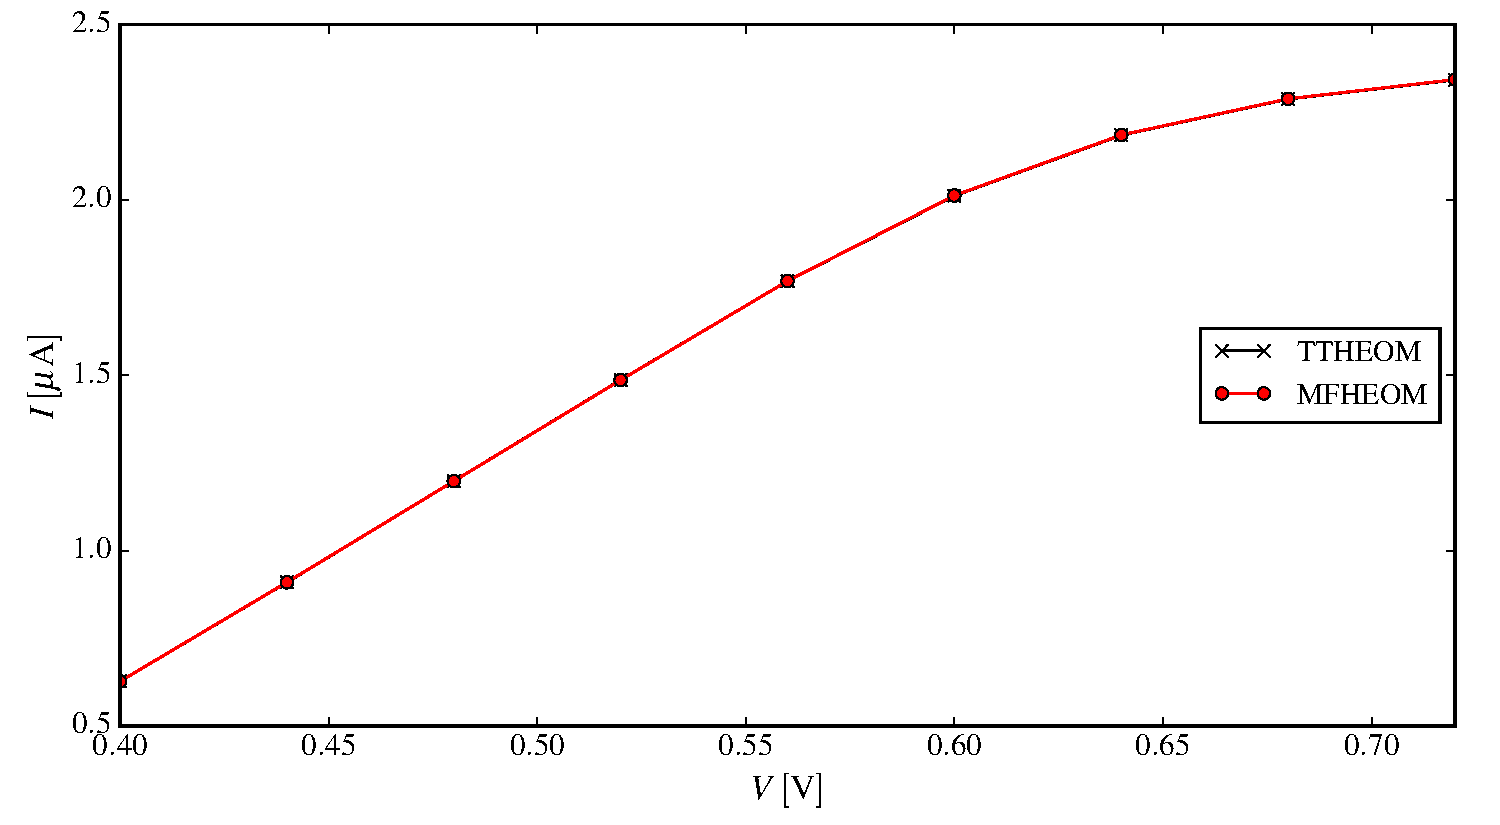
\includegraphics[width=0.8\textwidth]{figs/Peierls_L2_w0_0.1_t1_0.004_I_V_comparison.pdf}
\end{figure}
\clearpage
\subsection{$\omega_0 = \SI{50}{\milli\electronvolt}, t_1=\SI{20}{\milli\electronvolt}$}
\begin{figure}[!h]
	\centering
	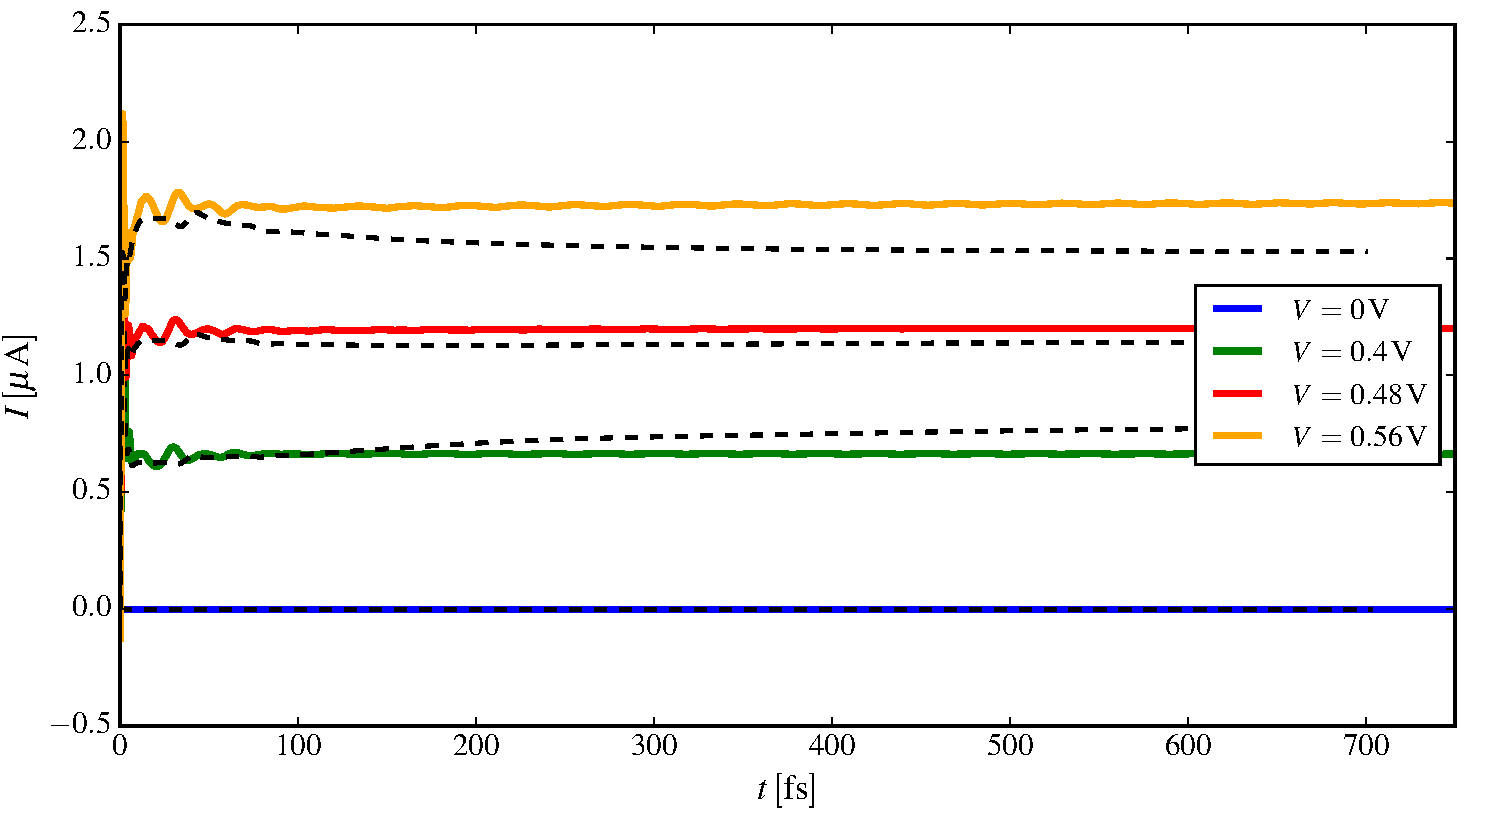
\includegraphics[width=0.8\textwidth]{figs/Peierls_L2_w0_0.05_t1_0.02_Vvar_comparison_currents.pdf}
	\caption{Colored lines: MF-HEOM. Black dashed lines: TT-HEOM}
\end{figure}
\begin{figure}[!h]
	\centering
	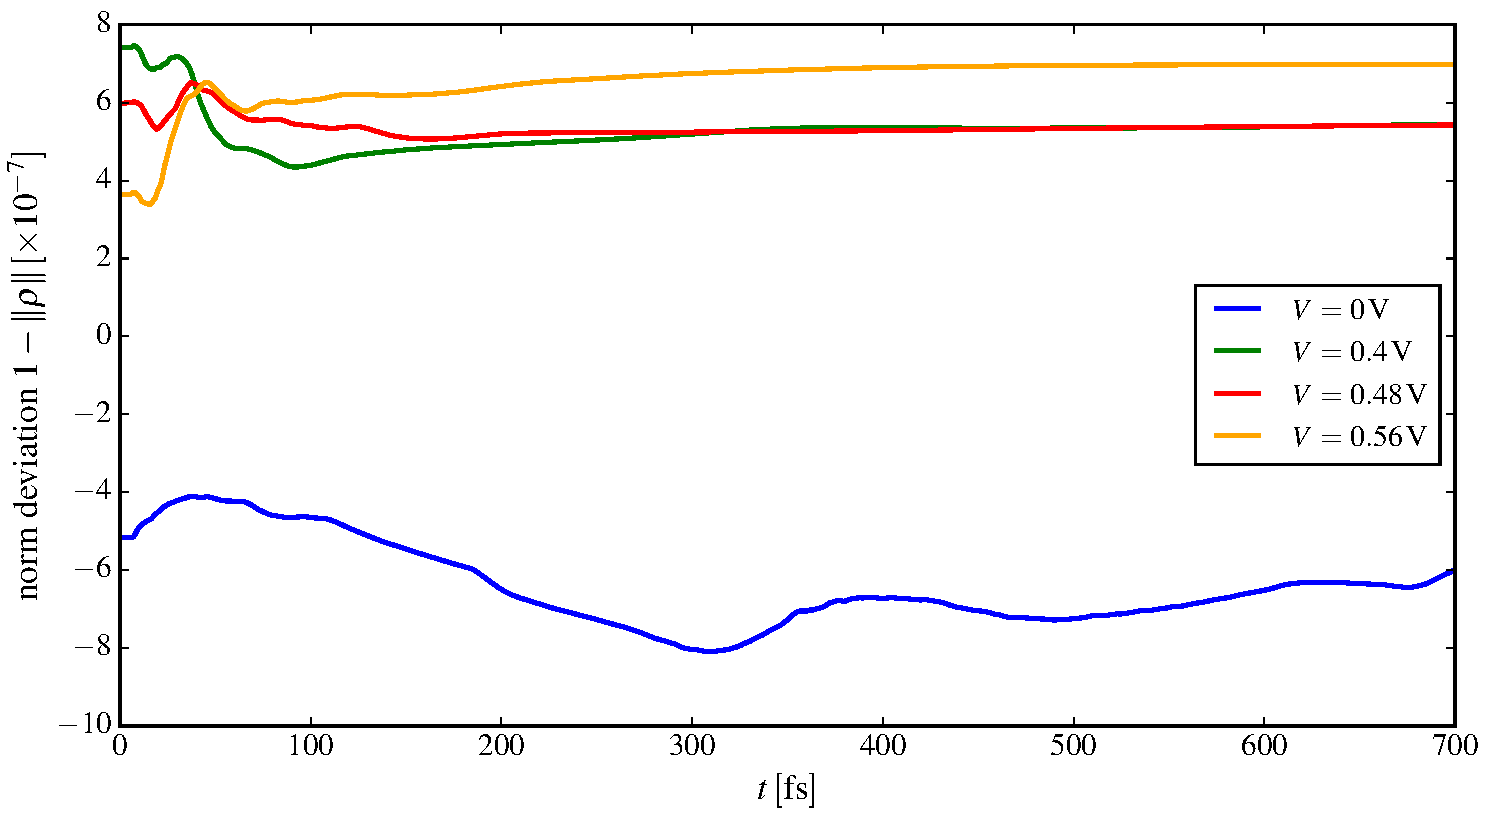
\includegraphics[width=0.8\textwidth]{figs/Peierls_L2_w0_0.05_t1_0.02_Vvar_norm.pdf}
\end{figure}
\begin{figure}[!h]
	\centering
	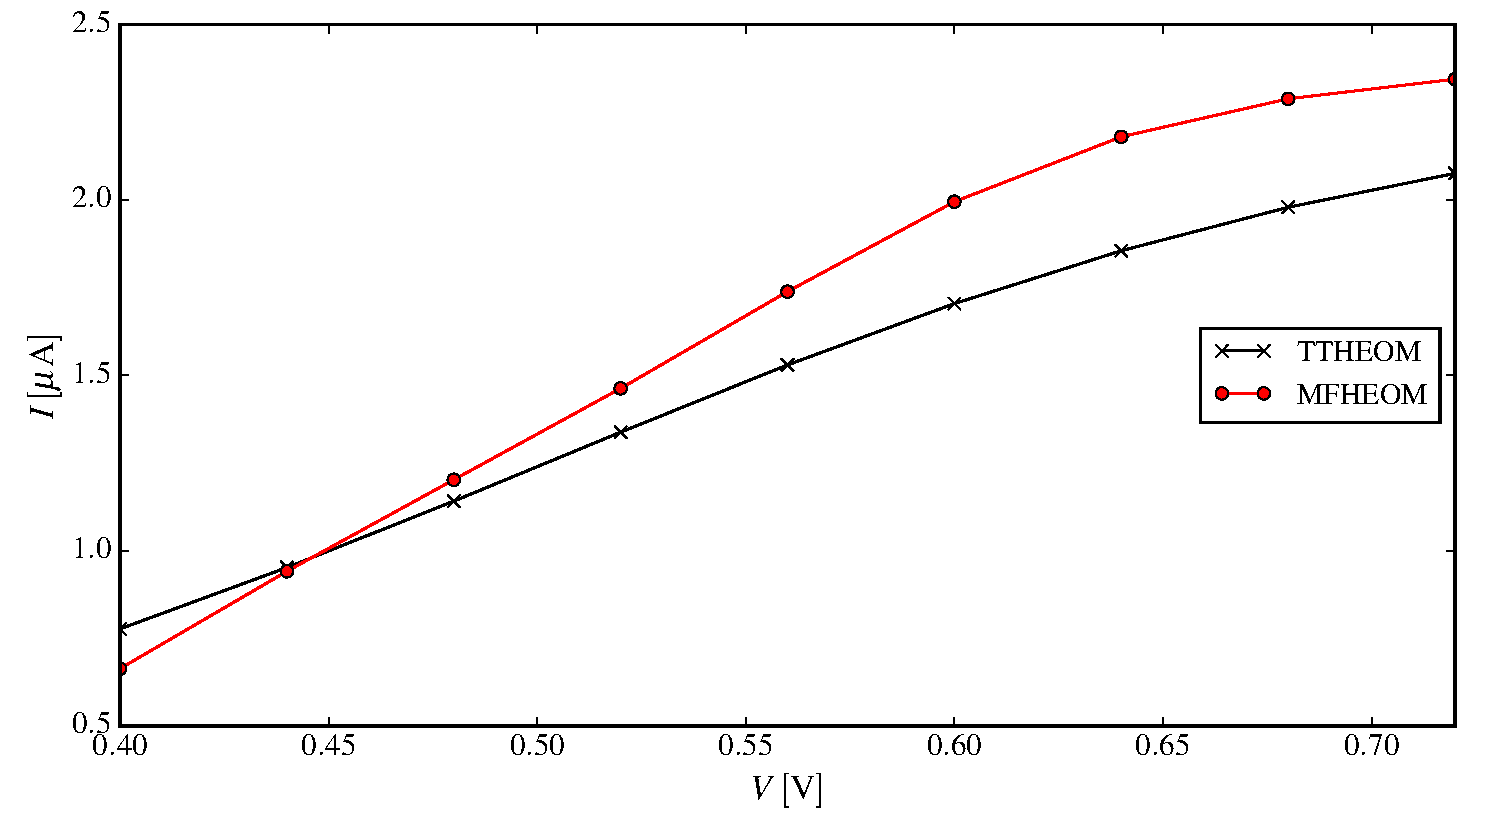
\includegraphics[width=0.8\textwidth]{figs/Peierls_L2_w0_0.05_t1_0.02_I_V_comparison.pdf}
\end{figure}
\clearpage
\subsection{$\omega_0 = \SI{100}{\milli\electronvolt}, t_1=\SI{20}{\milli\electronvolt}$}
\begin{figure}[!h]
	\centering
	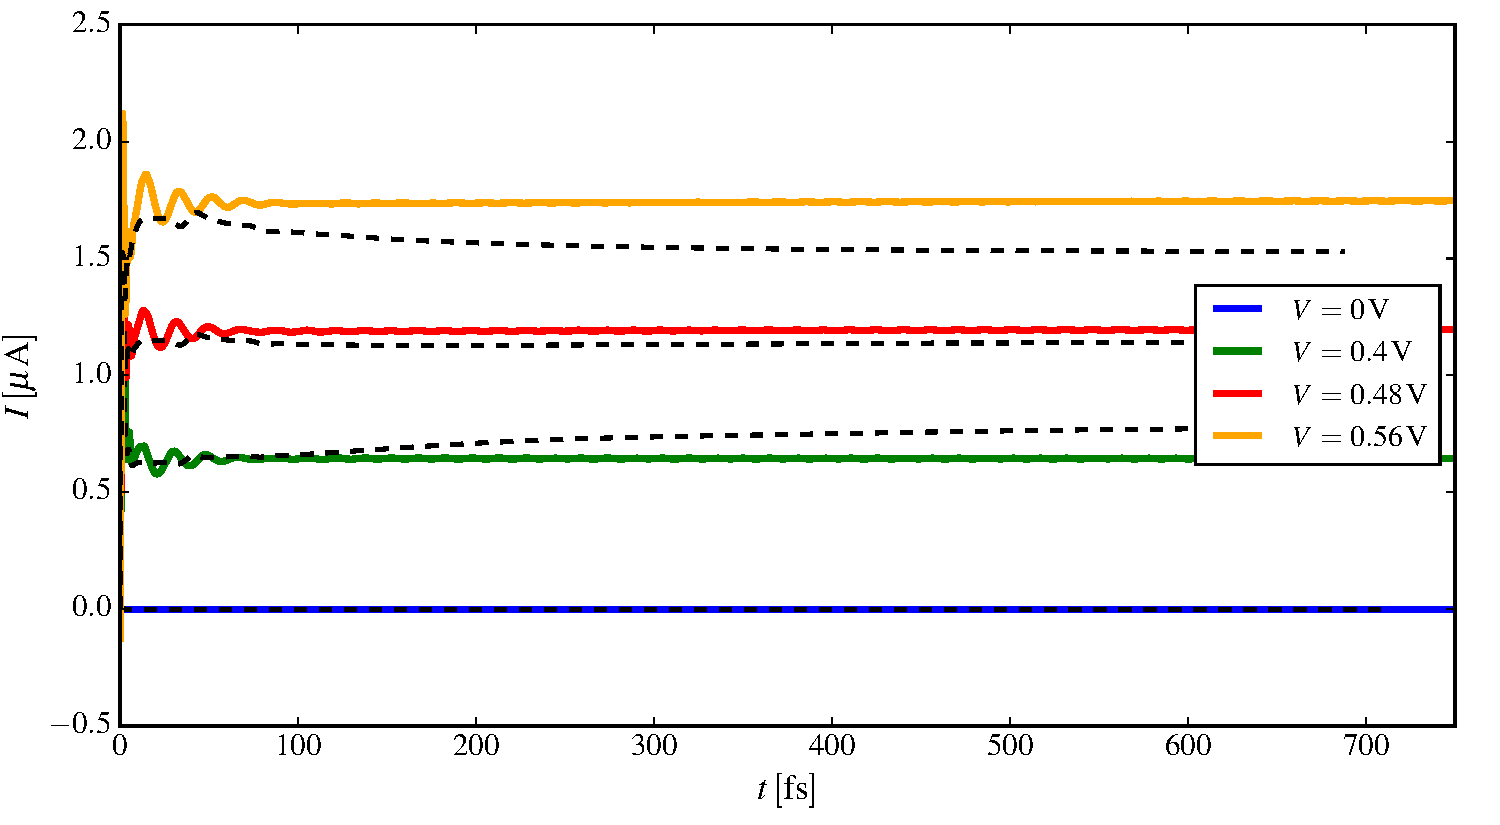
\includegraphics[width=0.8\textwidth]{figs/Peierls_L2_w0_0.1_t1_0.02_Vvar_comparison_currents.pdf}
	\caption{Colored lines: MF-HEOM. Black dashed lines: TT-HEOM}
\end{figure}
\begin{figure}[!h]
	\centering
	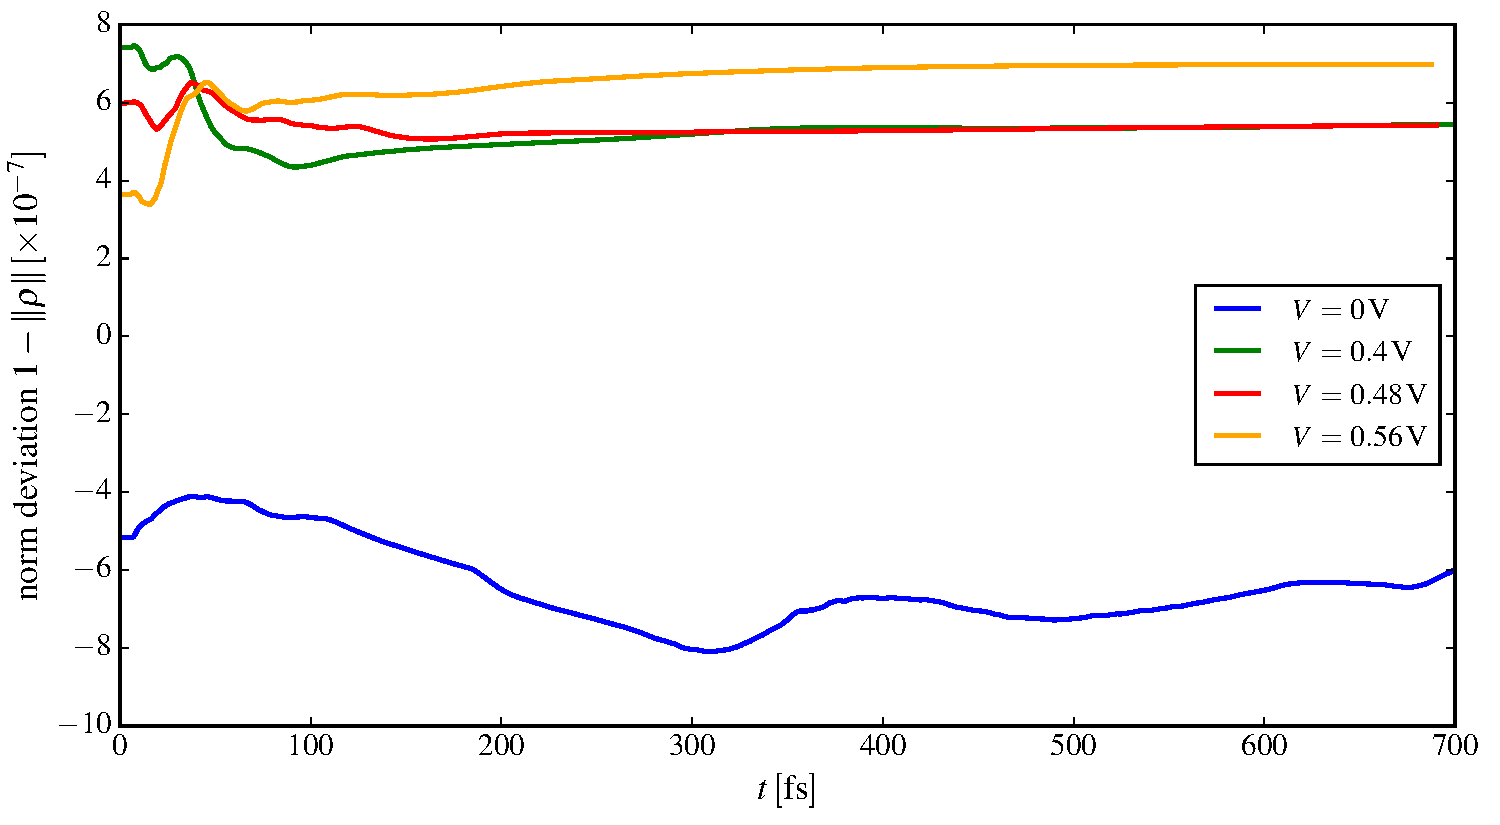
\includegraphics[width=0.8\textwidth]{figs/Peierls_L2_w0_0.1_t1_0.02_Vvar_norm.pdf}
\end{figure}
\begin{figure}[!h]
	\centering
	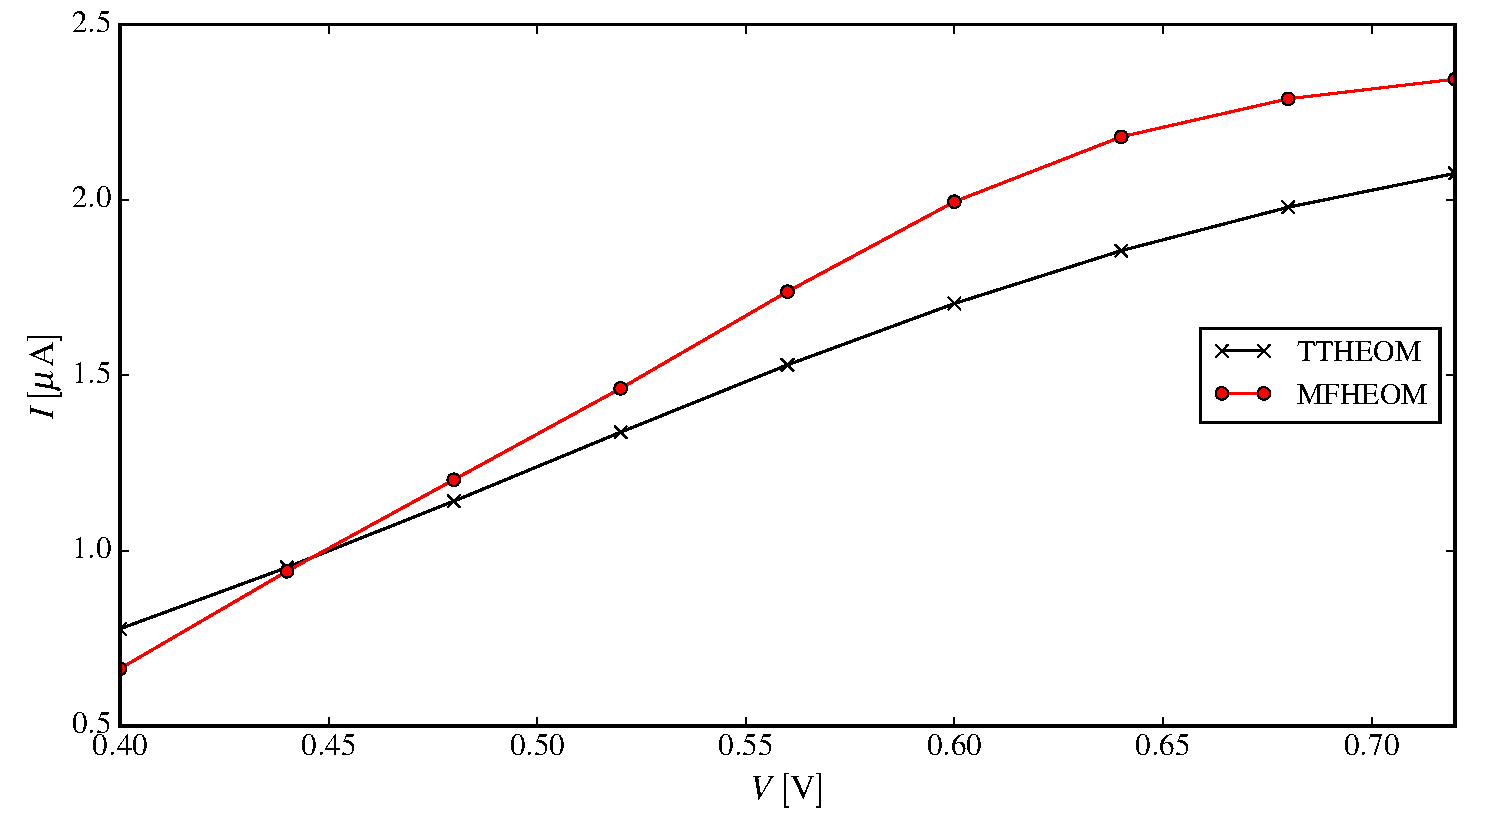
\includegraphics[width=0.8\textwidth]{figs/Peierls_L2_w0_0.1_t1_0.02_I_V_comparison.pdf}
\end{figure}
\section{Spinfull Peierls model $L=1\times 2$}
This system size corresponds to four electronic levels and one vibrational mode. The lead spin polarization is $P=0.5$ and the following plot is for checking convergence only. Here, $\omega=\SI{50}{\milli\electronvolt}$ and $t_1=\SI{20}{\milli\electronvolt}$.
\begin{figure}[!h]
	\centering
	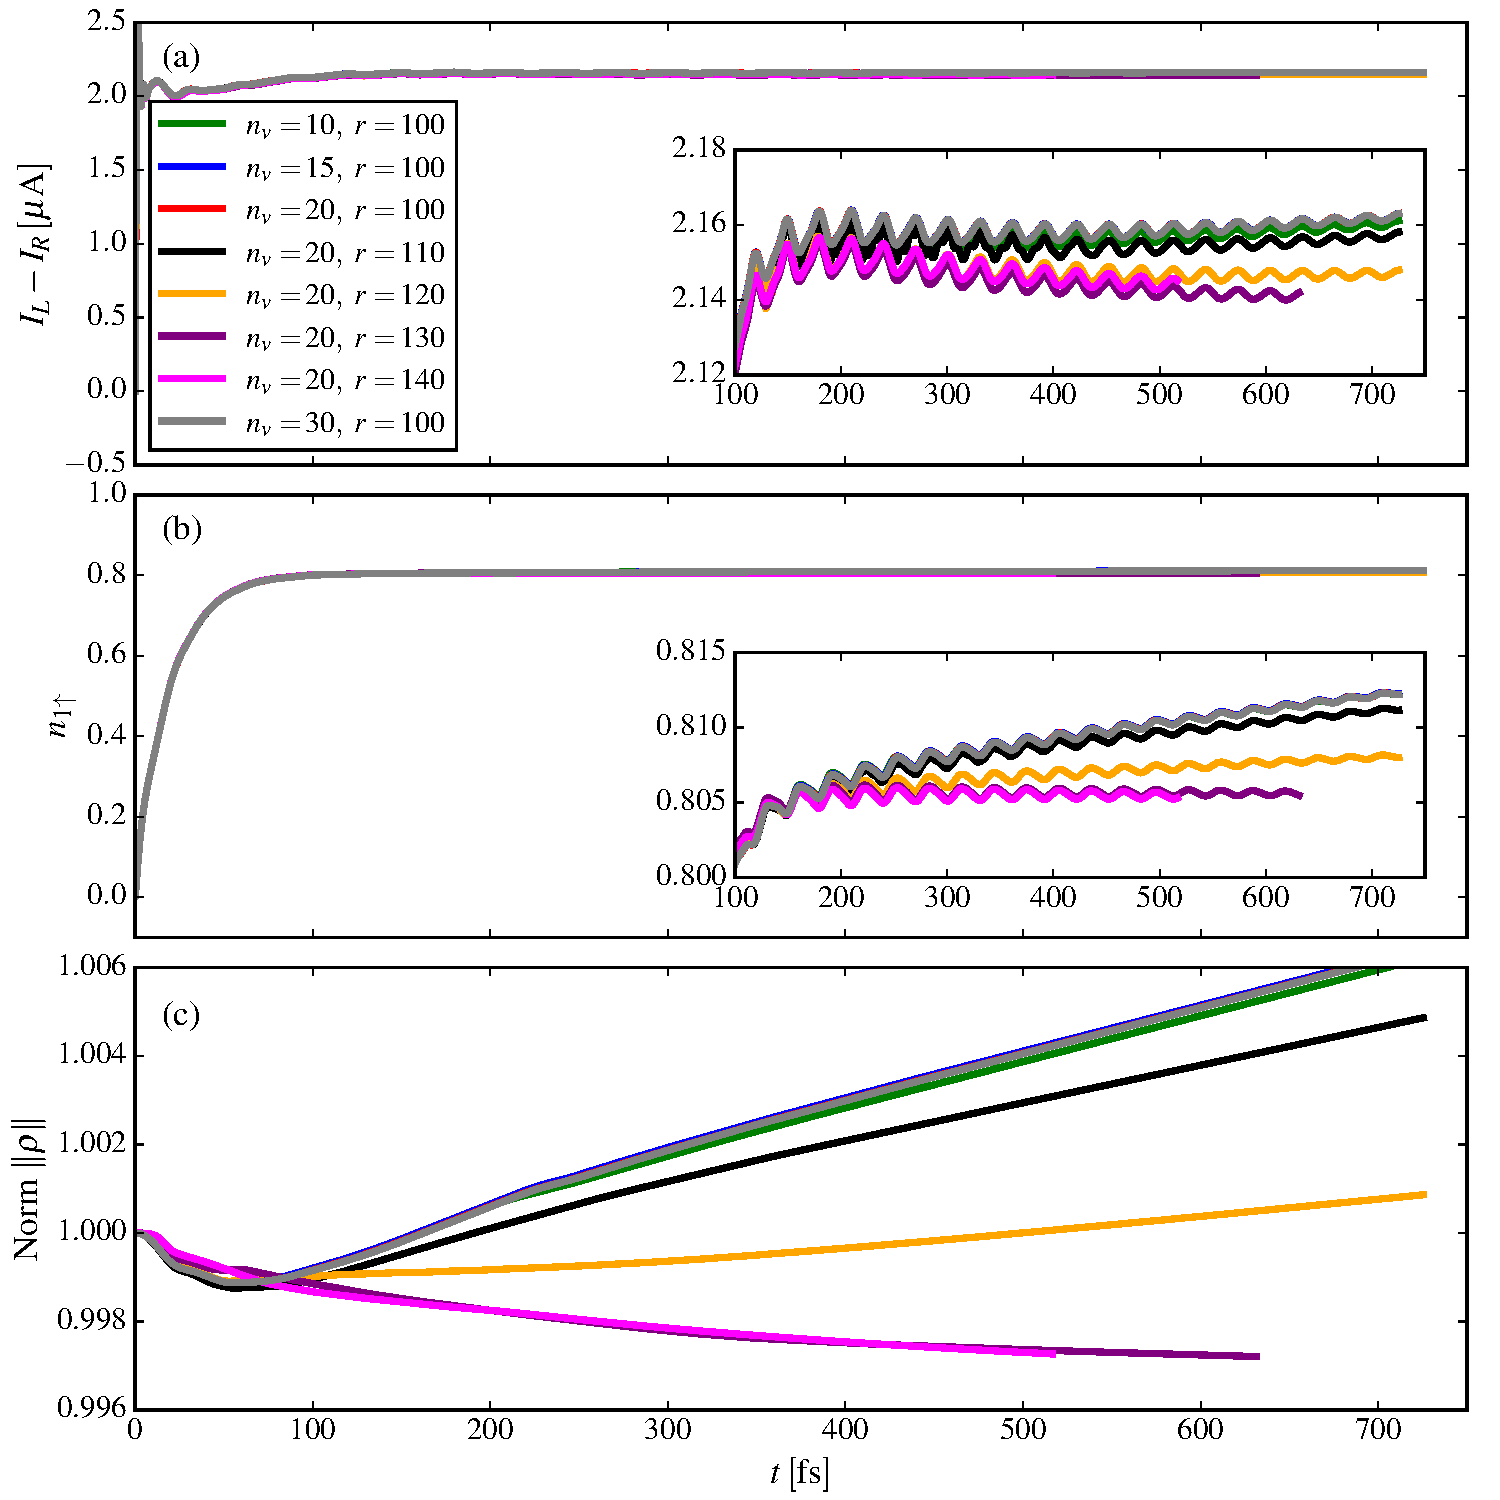
\includegraphics[width=1.0\textwidth]{figs/Convergence_TTHEOM_Fransson_1x2_w0_0.05_V0.48_P0.5_norm.pdf}
	\caption{Peierls model with $L=2$: Symmetrized current (a), spin-up population on site 1 (b) and norm of density matrix (c) for the parameters discussed above.}
\end{figure}
\begin{itemize}
	\item Variation of rank and number of vibrational states: Results do not change much
	\item Tiny oscillations die out very slowly
	\item Data is converged with respect to $n_v$ already for $n_v=10$. Can be seen from results not changing at all when increasing $n_v$ but keeping $r$ fixed.
	\item Start simulations for larger rank $r>100$. A rank of $r=120$ looks like giving the best results in the shortest calculation time (6-08:43:36 for $\SI{725}{fs}$). 
\end{itemize}
\section{Fransson model $L=1\times 3$}
This system size corresponds to four electronic levels and one vibrational mode. The lead spin polarization is $P=0.5$ and the following plot is for checking convergence only. Here, $\omega=\SI{50}{\milli\electronvolt}$, $t_1=\SI{20}{\milli\electronvolt}$ and $\lambda_1=\SI{1}{\milli\electronvolt}$.
\begin{figure}[!h]
	\centering
	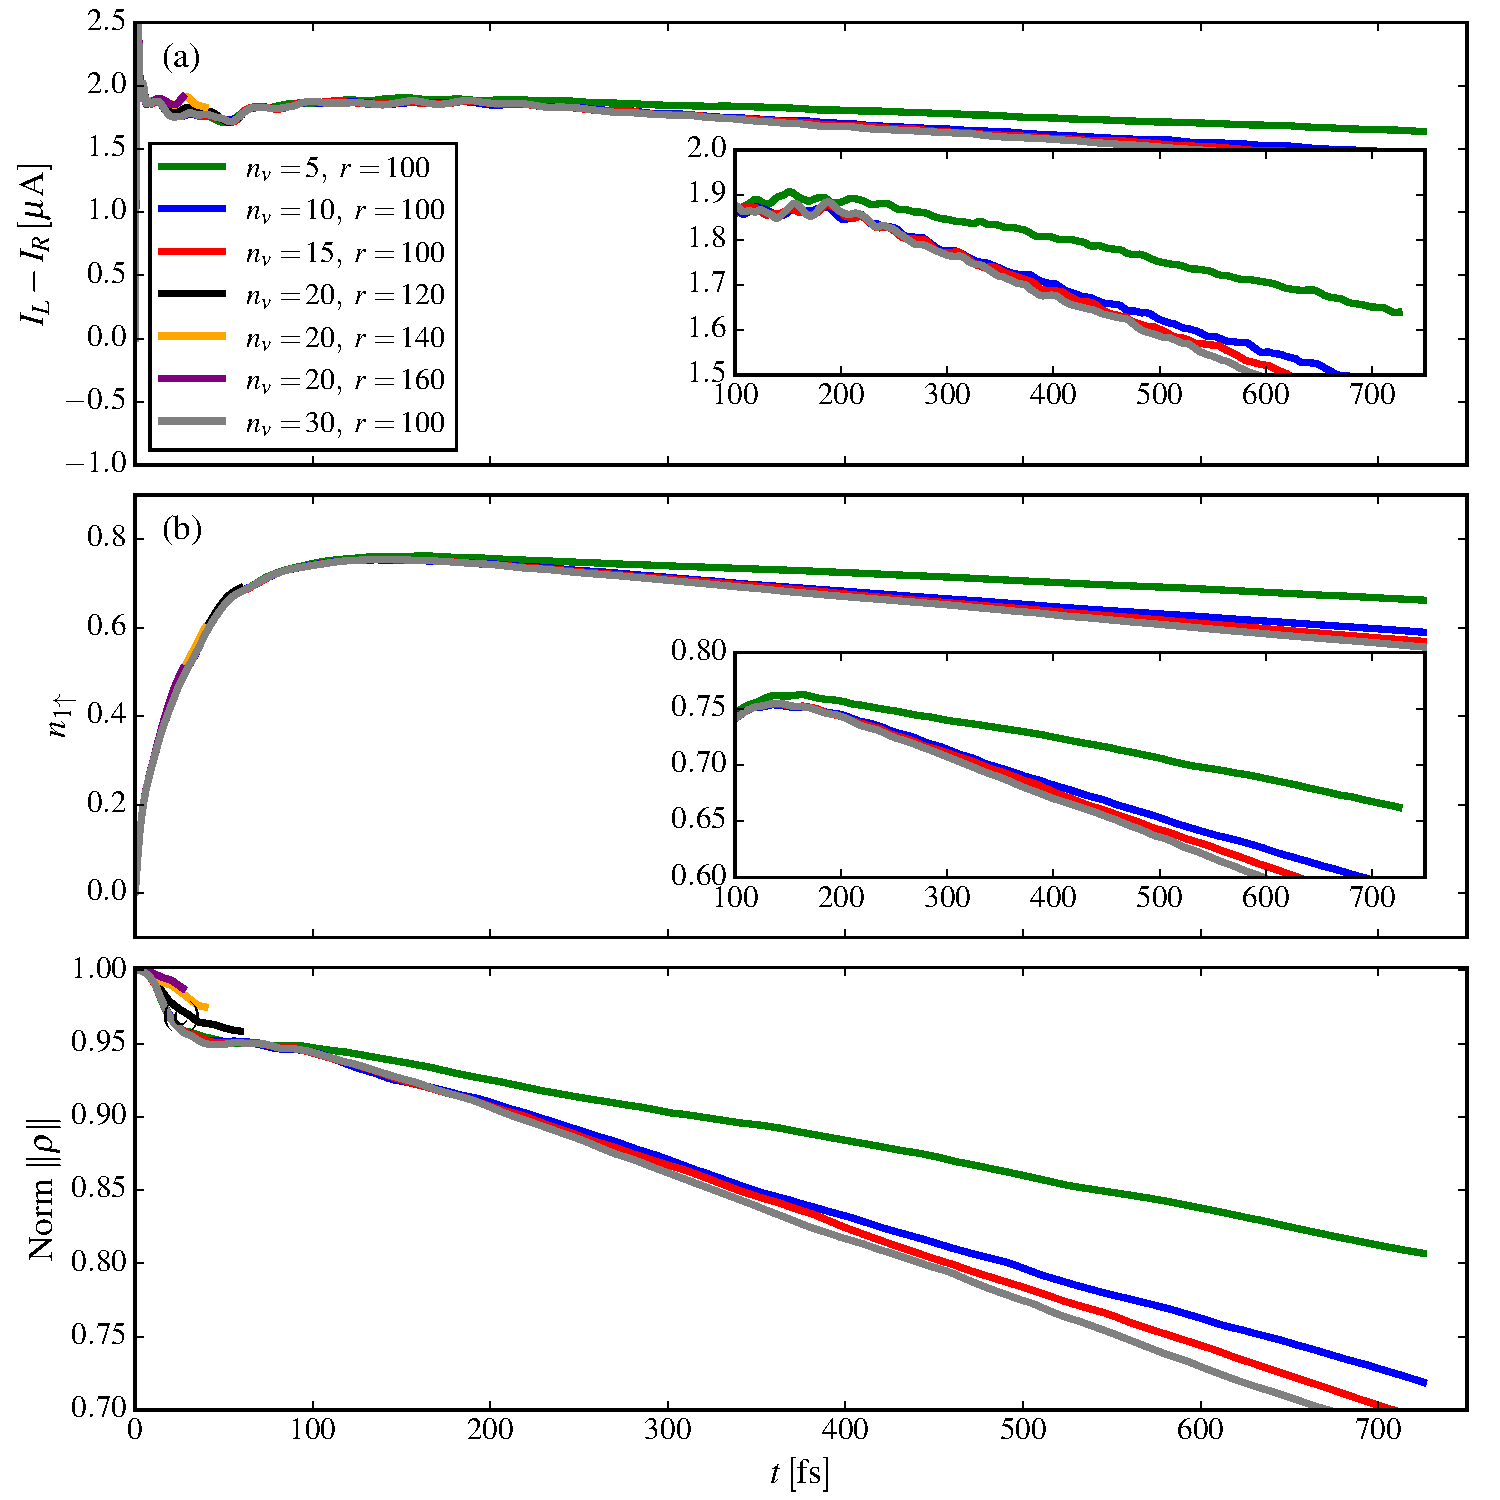
\includegraphics[width=1.0\textwidth]{figs/Convergence_TTHEOM_Fransson_1x3_w0_0.05_V0.48_P0.5_norm.pdf}
	\caption{Fransson model with $L=1\times 3$: Symmetrized current (a), spin-up population on site 1 (b) and norm of density matrix (c) for the parameters discussed above.}
\end{figure}\\
\begin{itemize}
	\item Results change quite a bit upon varying $n_v$ and $r$
	\item Seems like increasing $n_v$ while having $r$ fixed makes convergence worse
	\item Increasing the rank helps, but only short time data is available
	\item With old parameters, the norm was dropping down to $0.96$ for $r=100,n_v = 30$, while for the new parameters the norm drops down to $0.68$ for the same convergence parameters
\end{itemize}


\end{document}




